
%(BEGIN_QUESTION)
% Copyright 2014, Tony R. Kuphaldt, released under the Creative Commons Attribution License (v 1.0)
% This means you may do almost anything with this work of mine, so long as you give me proper credit

Analyze the following P\&ID segment showing a solenoid-controlled steam turbine start-up system (designed to ``back up'' an electric motor drive in the event the motor shuts down from power loss), explaining what will happen if either of the two solenoid valves loses electric power:

$$\includegraphics[width=15.5cm]{i04196x01.eps}$$

\vskip 10pt

Sketch arrows for both these solenoids showing the directions of air flow in their energized and de-energized states.  Must both solenoids change state to start the turbine (2oo2 to start), or is one sufficient (1oo2 to start)?

\vskip 20pt \vbox{\hrule \hbox{\strut \vrule{} {\bf Suggestions for Socratic discussion} \vrule} \hrule}

\begin{itemize}
\item{} What, exactly, is a {\it steam turbine} and what purpose does it serve in this system?
\item{} What practical purpose might a steam-driven turbine such as this serve in a process system, especially one ready to start up with one or more solenoids ``tripping''?
\item{} Explain the meaning of the letter ``R'' in the flag on the right-hand solenoid valve.
\end{itemize}

\underbar{file i04196}
%(END_QUESTION)




%(BEGIN_ANSWER)

If either solenoid loses electric power, it vents air pressure from the piston actuator of the fail-open steam valve, sending steam to the turbine to start it up:

$$\includegraphics[width=15.5cm]{i04196x02.eps}$$

%(END_ANSWER)





%(BEGIN_NOTES)

This is a 1oo2 to start system.

\vskip 20pt \vbox{\hrule \hbox{\strut \vrule{} {\bf Virtual Trip-testing} \vrule} \hrule}

This question is a good candidate for a ``Virtual Trip-testing'' exercise.  Presenting the diagram to students, you pose an assignment whereby students must figure out how to test some component of this system to check that it will operate as intended to shut down the system in an abnormal (trip) condition, with some realistic limitation (e.g. power cannot be shut off to the load).  Students then propose various methods for executing the test.  Your job is to determine whether or not their proposed tests will achieve the desired result(s).

During and after the exercise, it is good to ask students follow-up questions such as:

\begin{itemize}
\item{} Where might our planned test strategy go wrong?  In other words, what thing(s) might happen to foil our test, either to invalidate the results or to not honor the stated limitation(s)?
\item{} Suppose the limitation were different.  How would this affect our ability to carry out the test?
\item{} Is the last test strategy best one we could execute?
\end{itemize}


%INDEX% Final Control Elements, valve: fail-safe solenoids
%INDEX% Process: steam turbine auto-start 

%(END_NOTES)


